\documentclass{beamer}

\usepackage{graphicx,helvet,textpos,times,verbatim,tikz,enumerate,url}%
\usepackage{wrapfig}
\usepackage{color}
\usepackage{extarrows}
\usetheme{metropolis}           % Use metropolis theme


\usepackage{amsfonts,mathrsfs,pifont,bbding,pgfpages}
\usepackage[latin1]{inputenc}%
\usepackage[normalem]{ulem}
\usepackage{MnSymbol,wasysym}

% TikZ styles for drawing
\usetikzlibrary{intersections}
\usetikzlibrary{arrows,shapes,shadows,positioning,automata,patterns}
\usetikzlibrary{trees,snakes,decorations.pathmorphing,decorations.markings}
\usetikzlibrary{shapes.geometric,backgrounds,calc}

% TikZ styles for drawing
\tikzstyle{block} = [draw,rectangle,rounded corners,thick,minimum height=2em,minimum width=2em,fill=blue!20,draw=black!40]
\tikzstyle{block0} = [draw,rectangle,rounded corners,thick,minimum height=2em,minimum width=2em,fill=white!20,draw=white!90]
\tikzstyle{blockr} = [draw,rectangle,rounded corners,thick,rounded corners=6,thick,minimum height=2em,minimum width=2em,black!90,fill=gray!30]
\tikzstyle{sum} = [draw,circle,inner sep=0mm,minimum size=5mm,thick,fill=gray!40]
\tikzstyle{connector} = [->,thick]
\tikzstyle{blockex} = [draw,rectangle,rounded corners,thick,minimum height=2em,minimum width=2em,thick,fill=gray!20]
\tikzstyle{blockexg} = [draw,rectangle,rounded corners,thick,minimum height=2em,minimum width=2em,thick,fill=gray!20]
\tikzstyle{line} = [thick]
\tikzstyle{branch} = [circle,inner sep=0pt,minimum size=1mm,fill=black,draw=black,black]
\tikzstyle{branch2} = [circle,inner sep=0pt,minimum size=1mm,fill=black,draw=black]
\tikzstyle{guide} = [thick]
\tikzstyle{snakeline} = [connector, decorate, decoration={pre length=0.2cm,
                         post length=0.2cm, snake, amplitude=.4mm,
                         segment length=2mm},thick, ->]
\tikzstyle{place}=[circle,thick,draw=black!75,fill=gray!20,minimum size=6mm]%


\renewcommand{\vec}[1]{\ensuremath{\boldsymbol{#1}}} % bold vectors
\def \myneq {\skew{-2}\not =} % \neq alone skews the dash




\title{Applied Nonlinear Control \\
        \large Chapter 6 ~-~ Feedback Linearization}
\author{\large Shuai Qian}
\date{\today}
\institute{School of Automation \\
        Nanjing University of Science and Technology}


\begin{document}
  \maketitle

%contents---------------------------
  \begin{frame}
  \addtocounter{framenumber}{-2}
  \frametitle{Table of Contents}
  \thispagestyle{empty}
  \tableofcontents
  \end{frame}


  \section{1. Introduction}

  \begin{frame}{Introduction}
    \textbf{Central ideal of feedback linearization}
    \begin{itemize}
      \item Algebraically transform a nonlinear system dynamics into a (fully or partly) linear one, so that linear control techniques can be applied.
    \end{itemize}

    \textbf{Differences between feedback linearization and conventional linearization}
    \begin{itemize}
      \item \textcolor{red}{Feedback linearization} : achieved by exact state transformations and feedback.
      \item \textcolor{red}{Conventional linearization} (Jacobian linearization) : linear approximations of the dynamics.
    \end{itemize}
   \end{frame}


%--------------------------------
   \begin{frame}{Jacobian Linearization}

    Consider a nonlinear autonomous system (\ref{nonlinear})
    \begin{equation}\label{nonlinear}
      \dot{\vec{x}} = \vec{f(x)}
    \end{equation}
    Assume that $\vec{f(x)}$ is continuously differentiable,
    then the system can be written as
    $$
    \dot{\vec{x}} = (\frac{\partial \vec{f}}{\partial \vec{x}})_{\vec{x}=0} + \vec{f}_{h.o.t.}(\vec{x})
    $$
    (0 is an equilibrium point, and $\vec{f}(0) = 0$).
    Let $\vec{A}$ denotes the Jacobian matrix of $\vec{f}$ with respect to $\vec{x}$ at $\vec{x}=0$
    $$
    \vec{A} = (\frac{\partial \vec{f}}{\partial \vec{x}})_{\vec{x}=0}
    $$
    Then, the system
    $$
    \dot{\vec{x}} = \vec{Ax}
    $$
   \end{frame}


%---------------------------------
  \section{2. Intuitive Concepts}

  \begin{frame}{Example}
    Consider the control of the level $h$ of fluid in a tank (Figure \ref{tank}) to a specified level $h_{d}$.

    %place the figure and word together!
    \begin{wrapfigure}{l}{4cm}
    \vspace{-10pt}
    \includegraphics[width=4cm]{image/tank.pdf}\\
    \vspace{-15pt}
    \caption{Fluid level control in a tank}\label{tank}
    \vspace{-10pt}
    \end{wrapfigure}

    Variables:
    \begin{itemize}
      \item Control input : $u$
      \item Cross section of the tank : $A(h)$
      \item Cross section of the outlet \\ pipe : $a$
      \item Desired level : $h_{d}$
    \end{itemize}

    The dynamic model of the tank is
    \begin{equation}\label{dynamic}
      \frac{d}{dt}\left[\int_{0}^{h}A(h)dh\right] = u(t) - a \sqrt{2gh}
    \end{equation}

  \end{frame}


  \begin{frame}{Feedback Linearization}
  The dynamic (\ref{dynamic}) can be rewritten as
  $$ A(h)\dot{h} = u-a\sqrt{2gh} $$
  If we choose $u(t)$ as
  $$ 
  Origin~dynamic \quad \xrightarrow[linearization]{{\color{red} u(t) = a\sqrt{2gh} + A(h)v}} \quad \dot{h}=v
  $$

  with $v$ being an \textbf{``equivalent input"} to be specified.
  Chooseing $v$ as
  $$
   \dot{h}=v \quad \xrightarrow[close-loop]{{\color{red} v=-\alpha \widetilde{h}}} \quad \dot{h}+\alpha \widetilde{h}=0
  $$
  with $\widetilde{h} = h(t)-h_{d}$ being the \textbf{level error} ($\widetilde{h}(t)\rightarrow 0 ~\text{as}~ t \rightarrow \infty$), and $\alpha$ being a strictly positive constant.
  \end{frame}


  \begin{frame}{Feedback Linearization, ctd'}
  Finally, the actual input flow is determined by the nonlinear control law
  $$ u(t) = a\sqrt{2gh} - A(h)\alpha \widetilde{h} $$
    The idea of canceling the nonlinearities and imposing a desired linear dynamics, can be simply applied to a class of nonlinear systems described by the so-called \textbf{companion form, or controllability canonical form}:
    \begin{equation}\label{companion}
      x^{(n)} = f(\textbf{x}) + b(\textbf{x})u
    \end{equation}
    \vspace{-15pt}
    \begin{itemize}
      \item $u$ : scalar control input
      \item $x$ : scalar output of interest
      \item $\textbf{x} = \left[ x,\dot{x},\dots,x^{(n-1)}\right]^{T}$ : state vector
      \item $f(\textbf{x}), b(\textbf{x})$ : nonlinear functions of the states
    \end{itemize}
  \end{frame}


  \begin{frame}{Feedback Linearization, ctd'}
  In state-space representation, (\ref{companion}) can be written
  $$
  \frac{d}{dt}\left[\begin{array}{c}
                      x_{1} \\
                      \dots \\
                      x_{n-1} \\
                      x_{n}
                    \end{array}\right] = \left[\begin{array}{c}
                                                 x_{2} \\
                                                 \dots \\
                                                 x_{n} \\
                                                 f(\textbf{x}+b(\textbf{x})u)
                                               \end{array}\right]
  $$
  Using the control input ($b \neq 0$)\footnote{In our example, $b=\frac{1}{A(h)}, ~ f=-\frac{a\sqrt{2gh}}{A(h)}$}

  \begin{equation}\label{input}
    u = \frac{1}{b}\left[v-f\right]
  \end{equation}
  %(in example, $b=\frac{1}{A(h)}, ~ f=-\frac{a\sqrt{2gh}}{A(h)}$) \\
  we can cancel the nonlinearities and obtain the simple input-output relation
  $$ x^{(n)} = f(\textbf{x}) + b(\textbf{x})u \quad \xrightarrow[linearization]{E.q.(\ref{input})} \quad x^{(n)} = v $$
  \end{frame}


  \begin{frame}{Feedback Linearization, ctd'}
    Thus, the control law
    $$ v = -k_{0}x-k_{1}\dot{x}- \dots - k_{n-1}x^{(n-1)} $$
    with the $k_{i}$ chosen so that the polynomial $p^{n}+k_{n-1}p^{n-1} + \dots + k_{0}$ has all its roots strictly in the left-half complex plane, leads to the exponentially stable dynamics
    $$
    x^{n}+k_{n-1}x^{n-1}+\dots+k_{0}x = 0
    $$
    which implies that $x(t) \rightarrow 0$.
  \end{frame}

  \begin{frame}{Feedback Linearization, ctd'}
    For tasks involving the tracking of a desired output $x_{d}(t)$, the control law
    \begin{equation}\label{tracking}
      v = x_{d}^{(n)} - k_{0}e - k_{1}\dot{e}-\dots-k_{n-1}e^{(n-1)}
    \end{equation}
    where $e(t) = x(t)-x_{d}(t)$ is the tracking error, the control law leads to exponentially convergent tracking.
    \par \vspace{-5pt}
    \textcolor{red}{In our example}, $x_{d}(t)=h_{d}$ is constant, so choose
    $$v=-\alpha(h(t) - h_{d})$$
    with the $\alpha$ leads to the exponentially stable dynamics
    $$
    \dot{x} + \alpha x=0
    $$
    that is the polynomial $p+\alpha=0$ has all its roots strictly in the left-half complex plane
    $$
    p = -\alpha \quad \xrightarrow{p < 0} \quad \alpha > 0
    $$

  \end{frame}


  %-------------------------------------------
  \section{3. Input-State Linearization}

  \begin{frame}{Input-State Linearization}
    Consider the single-input nonlinear system
    $$ \dot{x} = f(x,u) $$
    The technique of \textbf{input-state linearization} solves this problem in two steps :
    \begin{enumerate}
      \item Find a \textbf{state transformation} $z=z(x)$, and an \textbf{input transformation} $u=u(x,v)$ :
          $$ \dot{x} = f(x,u) \quad \xrightarrow[u=u(x,v)]{z=z(x)} \quad \underbrace{\dot{z}=Az+bv}_{{\color{red}LTI}} $$
      \item Uses standard linear techniques (such as pole placement) to design $v$.
    \end{enumerate}
  \end{frame}


  \begin{frame}{Example}
  Consider the system with the equilibrium point $(0, 0)$

  \begin{equation}\label{input-state-example}
  \begin{aligned}
    \dot{x}_{1} &= -2x_{1}+ax_{2}+\underbrace{\sin x_{1}}_{nonlinearity} \\
    \dot{x}_{2} &= \underbrace{-x_{2}\cos x_{1} + u \cos(2x_{1})}_{nonlinearity}
  \end{aligned}
  \end{equation}

  Given the new set of state variables:
  $$ {\color{red} z_{1}=x_{1} , \quad z_{2}=ax_{2} + \sin x_{1}} $$

  then, the new state equations are
    \begin{equation}\label{new-state}
      \begin{aligned}
        \dot{z}_{1} &= -2 z_{1}+z_{2} \\
        \dot{z}_{2} &= -2 z_{1} \cos z_{1}+\cos z_{1} \sin z_{1}+a u \cos \left(2 z_{1}\right)
      \end{aligned}
    \end{equation}
  \end{frame}


  \begin{frame}{Example, ctd'}
  Now, the nonlinearities can be canceled by the control law of the form
  $$
    u=\frac{1}{a \cos \left(2 z_{1}\right)}\left(v-\cos z_{1} \sin z_{1}+2 z_{1} \cos z_{1}\right)
  $$
  where $v$ is an \textbf{equivalent input} to be designed, leading to a linear input-state relation
  \begin{equation}\label{input-state-relation}
    \begin{aligned}
      \dot{z}_{1} &= -2z_{1} + z_{2} \\
      \dot{z}_{2} &= v
    \end{aligned}
  \end{equation}
\begin{figure}
  \centering
    \begin{tikzpicture}[scale=0.5, auto, >=stealth']
      \matrix[ampersand replacement=\&, row sep=1cm, column sep=0.8cm]{
      \node [block] (origin) {$u \quad \xrightarrow{stabilize} \quad \text{original nonlinear system}$}; \\
      \node [block] (new) {$v \quad \xrightarrow{stabilize} \quad \text{new dynamics}$};\\
      };
      \draw [connector, very thick] ($(origin.south)$) --node{} (new);
    \end{tikzpicture}
    \end{figure}
  \end{frame}


\begin{frame}{Input-State Linearization, ctd'}
      The \textbf{closed-loop system} under the above control law is represented in the block diagram in Figure \ref{block}.
  \begin{figure}
  \centering
      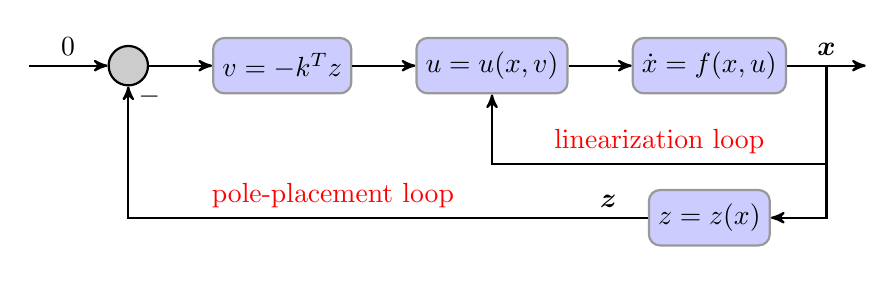
\begin{tikzpicture}[scale=0.5, auto, >=stealth']
      \matrix[ampersand replacement=\&, row sep=0.4cm, column sep=0.8cm]{

        \node[sum] (add) {};\&
        \node[block] (v) {$v=-k^{T}z$};\&
        \node[block] (u) {$u=u(x, v)$};\&
        \node[block] (dotx) {$\dot{x}=f(x,u)$}; \\
        \& \& \& \\
        \& \& \& \\
        \& \& \&
        \node[block] (z) {$z=z(x)$}; \\
        };

        %draw the lines
        \draw [connector, thick] ($(add.west)+(-2cm, 0cm)$) --node{0} ($(add.west)+(0cm, 0cm)$);
        \draw [connector, thick] ($(add.east)$) --node{} (v);
        \draw [connector, thick] ($(v.east)$) --node{} (u);
        \draw [connector, thick] ($(u.east)$) --node{} (dotx);
        \draw [connector, thick] ($(dotx.east)$) --node[above]{\vec{x}} ($(dotx.east)+(2cm, 0cm)$);
        \draw [connector, thick] ($(dotx.east)+(1cm, 0cm)$) |- ($(z.east)$);

        %for control the position of word, we can divide a line into segments!
        \draw [connector, thick] ($(z.west)$) -- node [above] {\vec{z}} ($(z.west)+(-2cm, 0cm)$) -- node [near end,above] {\textcolor{red}{ pole-placement loop}} ($(z.west)+(-10cm, 0cm)$) -| ($(add.south)+(0cm,-1cm)$) -- node [near end,right] {$-$} (add);
        \draw [connector, thick] ($(dotx.east)+(1cm, -2.5cm)$) -| node [near start,above] {\textcolor{red}{linearization loop}} (u);
      \end{tikzpicture}
  \caption{Input-State Linearization}
  \label{block}
  \end{figure}
\end{frame}


\begin{frame}{Remarks}
    A number of remarks can be made about the above control law:
    \begin{itemize}
      \item The result, though valid in a \textbf{large region} of the state space, is not global.($x_{1}=(\pi/4 + k\pi/2), k=1,2,\dots$)
      \item In order to implement the control law, ($z_{1}, z_{2}$) \textbf{must be available}. ~If they are not physically meaningful or cannot be measured directly, the \textbf{original state} $x$ must be measured and used to compute them.
      \item In general, we rely on the system model both for the \textbf{controller design} and for the \textbf{computation of} $\textbf{z}$.
    \end{itemize}
\end{frame}


%===============================
\section{4. Input-Output Linearization}


\begin{frame}{Input-Output Linearization}
Consider the tracking control problem, and the system
    \begin{equation}\label{tracking-control}
      \begin{aligned}
        \dot{\vec{x}} &= \vec{f}(\vec{x}, u) \\
        y &= h(\vec{x})
      \end{aligned}
    \end{equation}
The idea below constitutes the \textbf{intuitive basis} for the so-called \textbf{input-output linearization} approach to nonlinear control design:
    \begin{enumerate}
      \item \textcolor{red}{Objective} : make the output $y(t)$ track a desired trajectory $y_{d}(t)$ while keeping the whole state bounded.
      \item \textcolor{red}{Difficulty} : output $y$ is only indirectly related to the input $u$.
      \item \textcolor{red}{Try} : if we can find a direct and simple relation between the system output $y$ and the control input $u$ ?
    \end{enumerate}
\end{frame}


\begin{frame}{Example}
Consider the third-order system:
    \begin{equation}\label{third-order}
      \begin{aligned}
        \dot{x}_{1} &= \sin x_{2}+(x_{2}+1)x_{3} \\
        \dot{x}_{2} &= x_{1}^{5}+x_{3} \\
        \dot{x}_{3} &= x_{1}^{2}+u \\
        y &= x_{1}
      \end{aligned}
    \end{equation}
We find:
    $$
    \dot{y}=\dot{x}_{1}=\sin x_{2}+\left(x_{2}+1\right) x_{3}
    $$
    \begin{equation}\label{double}
      \ddot{y}=\left(x_{2}+1\right) u+f_{1}(x)
    \end{equation}
where $f_{1}(x)$ is a function of the state defined by
    \begin{equation}\label{f1x}
        f_{1}(x)=\left(x_{1}^{5}+x_{3}\right)\left(x_{3}+\cos x_{2}\right)+\left(x_{2}+1\right) x_{1}^{2}
    \end{equation}
\end{frame}


\begin{frame}{Example,ctd'}
    Clearly, (\ref{double}) represents an \textbf{explicit relationship} between $y$ and $u$.  If we choose the control input to be in the form
    $$
        E.q.(\ref{double}) \quad \xrightarrow[becomes]{ {\color{red}u=\frac{1}{x_{2}+1}\left(v-f_{1}\right)}} \quad \underbrace{\ddot{y} = v}_{linear~double-integrator}
    $$
   % $$
%       {\color{red}u=\frac{1}{x_{2}+1}\left(v-f_{1}\right)} \quad \xrightarrow[becomes]{E.q.(\ref{double})} \quad \underbrace{\ddot{y} = v}_{linear~double-integrator}
%    $$
Choosing $v$ as
\begin{equation}\label{choose-v}
  v = \ddot{y}_{d}-k_{1}e-k_{2}\dot{e}
\end{equation}
where $e=y(t)-y_{d}(t)$ be the \textbf{tracking error}, and $k_{1}, k_{2} > 0$.\\
So, the tracking error of the closed loop system is given by
$$
\ddot{e}+k_{2} \dot{e}+k_{1} e=0
$$
which represents an \textbf{exponentially stable} error dynamics. 
\end{frame}


\end{document}









